% SPDX-FileCopyrightText: 2025 Yifan Zhu <fanzhuyifan@gmail.com>
% SPDX-License-Identifier: CC0-1.0
\documentclass[8pt]{beamer}

\usepackage{tikz}
\usetikzlibrary{patterns} % LaTeX and plain TeX when using TikZ

\newcommand{\questionMark}{\usefont{T1}{cmr}{m}{n}\selectfont\color{red}{?}}

\title{moveResize restriction algorithm}

\begin{document}

\begin{frame}
  \maketitle
\end{frame}

\begin{frame}
  \only<1>{
    The big rectangle represents the overall available area -- windows are not visible outside.
    The grey rectangles represent the struts (think of them as obstacles -- windows are not visible in these areas).
  }
  \only<2>{
    Since the titlebar need to have certain number of continuous visible pixels, extend each strut to the left (by requiredPixels) and to the top (by titlebarHeight).
    Shrink the overall available area from the right and bottom by the same amount.
    These are the areas where the top left corner of the visible titlebar subrect cannot be placed (red diagonal lines).
    The remaining white area is availableRegion.
  }
  \only<3>{
    Since availableRegion is a QRegion, it is automatically split into rectangles (green with dashed borders, and ``availableRect'' in center).
  }
  \only<4>{
    The next step depends on window location (shown in blue) and move/resize type.
  }
  \only<5>{
    \frametitle{Move}
    Assume \emph{move} for now.
    Recall availableRect stores possible locations of the top left corner of the visible titlebar subrect.
    For each availableRect (stopping early if availableRect becomes empty):
    \begin{itemize}
    \item Apply restrictions to visible subrect top-left
      \begin{itemize}
      \item None needed for move.
      \end{itemize}
    \item Convert visible subrect top-left to window top-left
      \begin{itemize}
      \item 
        Extend each availableRect to the left by windowWidth - requiredPixels (gray dots, with text anchor candidate).
      \end{itemize}
    \end{itemize}

    For proposed anchor point (top left corner of the window, calculated from user input, red question mark), find closest anchor candidate point (green circle).
  }
  \only<6>{
    \frametitle{Move}
    We can visually inspect the solution.
  }
  \only<7>{
    \frametitle{Resize Left}
    Now assume user is resizing the \emph{left} of the window.
    For this case anchor is also top left.
    For each availableRect (stopping early if availableRect becomes empty):
    \begin{itemize}
    \item Apply restrictions to visible subrect top-left
      \begin{itemize}
      \item clip bottom to windowBottom - titlebarHeight (always performed for resize);
      \item clip right to windowRight - requiredPixels;
      \end{itemize}
    \item Convert visible subrect top-left to window top-left
      \begin{itemize}
      \item extend left to overall available area left.
      \end{itemize}
    \end{itemize}
    For proposed anchor point (red question mark), find closest anchor candidate point (green circle), while only allowing horizontal movement.
  }
  \only<8>{
    \frametitle{Resize Left}
    We can visually inspect the solution.
  }
  \only<9>{
    \frametitle{Resize Top Right}
    Now assume user is resizing the \emph{top right} of the window.
    For this case anchor is top right.
    Transform availableRect and convert to possible locations of the top right corner of the window.
    For each availableRect (stopping early if availableRect becomes empty):
    \begin{itemize}
    \item Apply restrictions to visible subrect top-left
      \begin{itemize}
      \item clip bottom to windowBottom - titlebarHeight (always performed for resize);
      \item clip left to windowLeft (top-left of visible subrect must be right of windowLeft);
      \end{itemize}
    \item Convert visible subrect top-left to window top-right:
      \begin{itemize}
      \item extend right to overall available area right;
      \item move left right by requiredPixels;
      \end{itemize}
    \end{itemize}
    For proposed anchor point (red question mark), find closest anchor candidate point (green circle).
  }
  \only<10>{
    \frametitle{Resize Top Right}
    We can visually inspect the solution.
  }

  \vfill

  \begin{center}
    \resizebox{0.8\textwidth}{!}{
      \begin{tikzpicture}[yscale=-1,every node/.style={scale=1.5,thick}]

        % Draw the main blank rectangle canvas
        \draw[thick] (0,0) rectangle (16,12);
        \tikzstyle{strut} = [fill=gray!30, draw=black, thick]
        \tikzstyle{forbidden} = [
        draw=black, thick, fill opacity=0.3, text opacity=1, pattern=north east lines, pattern color=red]
        \tikzstyle{available} = [fill=green!30, dashed, fill opacity=.3, text opacity=1, draw=black, thick]
        \tikzstyle{window} = [fill=blue!50, fill opacity=.5, text opacity=1, draw=black, thick]
        \tikzstyle{final} = [
        draw=black, thick, fill opacity=0.3, text opacity=1, pattern=dots, pattern color=black]
        \tikzstyle{result} = [green, fill=green, radius=0.15cm]
        \tikzstyle{windowFinal} = [fill opacity=.3, text opacity=1, draw=black, thick, pattern=north west lines, pattern color=blue]

        \only<1-3,6,8,10>{
          % Draw rectangles on four sides
          \draw[strut] (6,0) rectangle (10,1);
          \draw[strut] (6,11) rectangle (10,12);
          \draw[strut] (0,2) rectangle (1,10);
          \draw[strut] (15,3) rectangle (16,9);

          % \draw node at (8, 6) {Screen};

          \draw[strut] (17,0) rectangle (19,1) node[midway] {Strut}; 
        }

        \only<2-3>{
          \draw[forbidden] (17,1) rectangle (20,2) node[midway] {Visible subrect};
          \draw[forbidden] (3,-1) rectangle (10,1);
          \draw[forbidden] (3,10) rectangle (10,12);
          \draw[forbidden] (-3,1) rectangle (1,10);
          \draw[forbidden] (12,2) rectangle (16,9);

          \draw[forbidden] (13,0) rectangle (16,12);
          \draw[forbidden] (0,11) rectangle (16,12);
        }
        \only<3-4>{
          \draw[available] (17,2) rectangle (21,3) node[midway] {availableRect};
          \draw[available] (0,0) rectangle (3,1) node[midway] {availableRect};
          \draw[available] (0,10) rectangle (3,11) node[midway] {availableRect};
          \draw[available] (10,0) rectangle (13,2) node[midway] {availableRect};
          \draw[available] (10,9) rectangle (13,11) node[midway] {availableRect};
          \draw[available] (1,1) rectangle (10,10) node[midway] {availableRect};
          \draw[available] (10,2) rectangle (12,9) node[midway,align=left] {available\\Rect};
        }
        \only<5,7,9>{
          \draw[available] (17,2) rectangle (21,3) node[midway] {availableRect};
          \draw[available] (0,0) rectangle (3,1);
          \draw[available] (0,10) rectangle (3,11);
          \draw[available] (10,0) rectangle (13,2);
          \draw[available] (10,9) rectangle (13,11);
          \draw[available] (1,1) rectangle (10,10);
          \draw[available] (10,2) rectangle (12,9);
        }
        \only<4->{
          \draw[window] (17,3) rectangle (19,4) node[midway] {Window};
          \draw[window] (5, 4) rectangle (13, 8) node[midway] {Window};
        }
        \only<5>{
          \draw[final] (17,4) rectangle (21,5) node[midway] {anchor candidate};
          \draw[final] (-5,0) rectangle (3,1) node[midway] {anchor candidate};
          \draw[final] (-5,10) rectangle (3,11) node[midway] {anchor candidate};
          \draw[final] (5,0) rectangle (13,2) node[midway] {anchor candidate};
          \draw[final] (5,9) rectangle (13,11) node[midway] {anchor candidate};
          \draw[final] (-4,1) rectangle (10,10) node[midway] {anchor candidate};
          \draw[final] (5,2) rectangle (12,9) node[midway,align=left] {anchor candidate};
          \draw node at (19, 5.5) {\questionMark : proposed anchor};
          \draw node at (14, 8) {\questionMark};
          \draw[result] (18, 6.5) circle node[right] {closestPoint};
          \draw[result] (13, 9) circle;
        }
        \only<6>{
          \draw node at (19, 5.5) {\questionMark : proposed anchor};
          \draw node at (14, 8) {\questionMark};
          \draw[result] (18, 6.5) circle node[right] {closestPoint};
          \draw[result] (13, 9) circle;
          \draw[windowFinal] (17,7) rectangle (20,8) node[midway] {Final Window};
          \draw[windowFinal] (13, 9) rectangle (21, 13) node[midway] {Final Window};
        }
        \only<7>{
          \draw[final] (17,4) rectangle (21,5) node[midway] {anchor candidate};
          \draw[final] (0,0) rectangle (3,1) node[midway] {anchor candidate};
          % \draw[final] (0,10) rectangle (3,11) node[midway] {anchor candidate};
          \draw[final] (0,1) rectangle (10,7) node[midway] {anchor candidate};
          \draw node at (19, 5.5) {\questionMark : proposed anchor};
          \draw node at (11, 4) {\questionMark};
          \draw[result] (18, 6.5) circle node[right] {closestPoint};
          \draw[result] (10, 4) circle;
        }
        \only<8>{
          \draw node at (19, 5.5) {\questionMark : proposed anchor};
          \draw node at (11, 4) {\questionMark};
          \draw[result] (18, 6.5) circle node[right] {closestPoint};
          \draw[result] (10, 4) circle;
          \draw[windowFinal] (17,7) rectangle (20,8) node[midway] {Final Window};
          \draw[windowFinal] (10, 4) rectangle (13, 8) node[midway] {Final Window};
        }
        \only<9>{
          \draw[final] (17,4) rectangle (21,5) node[midway] {anchor candidate};
          % \draw[final] (0,0) rectangle (3,1) node[midway] {anchor candidate};
          % \draw[final] (0,10) rectangle (3,11) node[midway] {anchor candidate};
          \draw[final] (13,0) rectangle (16,2) node[midway] {anchor candidate};
          % \draw[final] (10,9) rectangle (13,11) node[midway] {anchor candidate};
          \draw[final] (8,1) rectangle (16,7) node[midway] {anchor candidate};
          \draw[final] (13,2) rectangle (16,7) node[midway,align=left] {anchor candidate};
          \draw node at (19, 5.5) {\questionMark : proposed anchor};
          \draw node at (11, 0) {\questionMark};
          \draw[result] (18, 6.5) circle node[right] {closestPoint};
          \draw[result] (11, 1) circle;
        }
        \only<10>{
          \draw node at (19, 5.5) {\questionMark : proposed anchor};
          \draw node at (11, 0) {\questionMark};
          \draw[result] (18, 6.5) circle node[right] {closestPoint};
          \draw[result] (11, 1) circle;
          \draw[windowFinal] (17,7) rectangle (20,8) node[midway] {Final Window};
          \draw[windowFinal] (5, 1) rectangle (11, 8) node[midway] {Final Window};
        }
      \end{tikzpicture}
    }
  \end{center}
\end{frame}

\end{document}
